

\begin{appendices}

\chapter*{Appendices}
\addcontentsline{toc}{chapter}{Appendices}
% Additional appendices can be added here
\section{List of Abbreviations}
% \newacronym{kgs}{KGs}{Knowledge Graphs}
% \newacronym{nlp}{NLP}{Natural Language Processing}
% \acro{ecu}[ECU]{European currency unit}
% \begin{acronym}[ECU]


% \chapter*{List of abbreviations} \label{LOA}
\begin{acronym}
\acro{kg}[KG]{Knowledge graph}
\acro{kb}[KB]{Knowledge base}
\acro{qe}[QE]{Questioning Engine}
\acro{nlp}[NLP]{Natural Language Processing}

\acro{qg}[QG]{Question generation}

\acro{ner}[NER]{Named Entity Recognition}
\acro{adp}[adp]{adposition}
\acro{pobj}[pobj]{prepositional object}
\acro{dobj}[dobj]{direct object}
\acro{nsubj}[nsubj]{nominal subject}
\acro{conj}[conj]{coordinating conjunction}
\acro{amod}[amod]{adjectival modifier}
\acro{POS}[POS]{part of speech}
\acro{pron}[pron]{pronoun}
\acro{SRO}[SRO]{subject,relation and object}
\acro{Tf-Idf}[Tf-Idf]{Term frequency-Inverse document frequency}
\acro{Tf}[Tf-Idf]{Term frequency}
\acro{Idf}[Idf]{Inverse document frequency}
\acro{KNN}[KNN]{\textit{k} -Nearest Neighbors}
\acro{RNN}[RNN]{Recurrent Neural Network}
\acro{ALL}[ALL]{Adaptive LogSoftmax with Loss}
\acro{NLLLoss}[NLLLoss]{Negative log likelihood loss}
\acro{BPTT}[BPTT]{Back Propagation through time}
\acro{DAG}[DAG]{directed acyclic graph }
\acro{SGD}[SGD]{Stochastic gradient descent }
\acro{CLR}[CLR]{Cyclic learning rate }
\acro{LTR}[LTR]{Learn to Rank }
\acro{IR}[IR]{Information Retrieval }
\acro{AI}[AI]{Artificial Intelligence }
\acro{PMF}[PMF]{Probability Mass Function }
\acro{MSE}[MSE]{Mean Squared Error}
\acro{GAN}[GAN]{generative adversarial network}
\acro{PIM}[PIM]{Product Information Management}
\acro{SKU}[SKU]{stock-keeping unit}

\acro{SEO}[SEO]{Search Engine Optimization}

\end{acronym}


\section{Appendix A}
For this project, python client elasticsearch 6.8.2 is installed as the client needs to be compatible with Elastic search version being used. The official Python client provides mapping with Elasticsearch REST APIs.

\begin{lstlisting}[language=Python,caption={Elastic search},label={code:es_search}]
    resp=self.es.search("english-name-category",{"_source":["id","name","category"],
    'from':_from,
    'size' :_size ,
    "query": {"match_all": {}}})
    \end{lstlisting}
% Content for Appendix A goes here...

\subsection*{Confusion matrix}
\begin{lstlisting}[language=Python,caption={Confusion matrix},label={code:confusion matrix}]
def confusionMatix(self,df_en):
# Keep track of correct guesses in a confusion matrix
data = Data(df_en)
n_categories = len(data.all_category)

batch = random.choices(data.all_category,k=20)

confusion = torch.zeros(n_categories, n_categories)
n_confusion = 10000

# Go through a bunch of examples and record which are correctly guessed
for i in range(n_confusion):
    category, name, category_tensor, name_tensor = data.randomTrainingExample()
    if category in batch:
        output = self.evaluate(name_tensor)
        guess, guess_i = data.categoryFromOutput(output)
        category_i =data.all_category.index(category)
        confusion[category_i][guess_i] += 1

# Normalize by dividing every row by its sum
for i in range(20):
    confusion[i] = confusion[i] / confusion[i].sum()


# Set up plot
fig = plt.figure()
ax = fig.add_subplot(111)
cax = ax.matshow(confusion.numpy())
fig.colorbar(cax)

# Set up axes
ax.set_xticklabels([''] + data.all_category, rotation=45)
ax.set_yticklabels([''] + data.all_category)

# Force label at every tick
ax.xaxis.set_major_locator(ticker.MultipleLocator(1))
ax.yaxis.set_major_locator(ticker.MultipleLocator(1))

# sphinx_gallery_thumbnail_number = 2
plt.show()
plt.savefig('confusion.png', dpi=400)

\end{lstlisting}

\subsection*{Load PyTorch model}
\begin{lstlisting}[language=Python,caption={Load PyTorch model},label={code:Loadpt}]
class Predict():
    def __init__(self):
         self.rnn = torch.load('ngram-rnn-classification.pt')
        \end{lstlisting}

\section{Appendix B}
\begin{figure}
    \centering    
    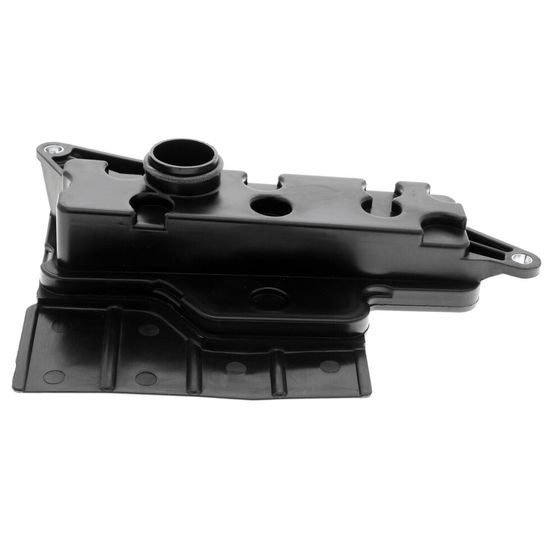
\includegraphics[scale=0.5]{ht_rm.jpg}
    \caption{Hydraulic filter automatic transmission VAICO V70-0613 for Lexus RX \parencite{RM}}
    \label{fig:sparepart}
\end{figure}

\end{appendices}
